\documentclass[12pt]{article}
\usepackage{fullpage}
\usepackage{graphicx, rotating, booktabs} 
\usepackage{times} 
\usepackage{fbb} 
\usepackage{natbib} 
\usepackage{indentfirst} 
\usepackage{setspace}
\usepackage{grffile} 
\usepackage{hyperref}
\usepackage{tikz-cd}
 \usetikzlibrary{cd}
\usepackage[export]{adjustbox}
\usepackage[most]{tcolorbox}
\usepackage{verbatimbox}
\usepackage{lscape}
\usepackage{afterpage}
\usepackage{amsmath}
\usepackage[labelfont={bf},textfont=it,labelsep=period]{caption}
 \usepackage{multirow} 
\setcitestyle{aysep{}}
\usepackage{dcolumn}

\hypersetup{
  colorlinks = true,
  urlcolor = blue,
  linkcolor = black,
  citecolor = black,
  pdfauthor = {Joshua Alley},
  pdfkeywords = {},
  pdftitle = {},
  pdfsubject = {},
  pdfpagemode = UseNone,
%  pdffitwindow = true
%  pdfcenterwindow = true
}



\singlespace
\title{\textbf{Arms and Electoral Influence: How Arms Deals with Autocracies Shape Defense Contracting in the United States}}
\author{Joshua Alley \\
Assistant Professor \\
University College Dublin\thanks{Thanks to Brian Blankenship, Rosella Capella, Jonathan Caverley, Jonathan Chu, Ben Fordham, Erik Lin-Greenberg, Zachary Markovitch, Leah Matchett, Andy Philips and Phil Potter, as well as participants in the Boston University Political Economy of Security Online Workshop Series and 2022 Meeting of the International Studies Association for helpful comments.} \\
joshua.alley@ucd.ie
}

 
\date{\today}

\bibliographystyle{apsr}

\usepackage{sectsty}
\sectionfont{\Large}
\subsectionfont{\noindent\large\textit}
\subsubsectionfont{\normalsize}

\makeatletter
\renewcommand\tiny{\@setfontsize\tiny{9}{10}}
\makeatother


\begin{document}

\maketitle 

\begin{abstract} 
As elections approach, U.S. leaders make additional arms deals with autocracies. 
U.S. leaders make these deals to help win elections by claiming credit for providing jobs and increasing defense contracting in swing states.
Autocratic arms recipients have greater political flexibility to strike arms deals near presidential elections and can increase their security. 
I provide three pieces of evidence for this argument.  
First, I detail electoral cycles in arms deals between the United States and autocracies. 
I then link arms deals to defense contract awards in swing states.
Finally, I provide additional evidence for the process by showing that U.S. allies drive most of the autocratic arms deals cycle and that the same platforms that move in arms deals increase swing state contracts.  
The argument and results help explain why U.S. security cooperation with autocracies endures despite normative and practical concerns.
\end{abstract} 



\newpage 
\doublespace 


\section{Introduction}



% US-Brazil 1972
In 1972, the Nixon administration struck ten deals to transfer or sell arms to Brazil.
Over the next four years, Brazil's military dictatorship received 500 M-113 armoured personnel carriers, five destroyers, seven submarines, and eight S-2E Tracker anti-submarine warfare aircraft.
These deals came while Nixon sought reelection and arms deliveries continued after his 1974 resignation. 


% Obama 2012
Something similar happened during the 2012 presidential election, when Saudi Arabia ordered arms from the Obama administration.\footnote{Obama first announced the deal in 2010.} 
Twelve deals included 400 Harpoon anti-ship missiles, 12 Apache attack helicopters, and 63 K-6 120mm mortars, along with F-15 jet parts, guided bombs, and other helicopters. 
Subsequent weapons deliveries spanned the next eight years, including the 2015 Saudi intervention in Yemen's civil war.\footnote{All deal information from \citep{SIPRI2021}.}


% puzzle/question 
The confluence of large arms deals with autocracies and presidential elections is not coincidental.
Domestic political competition in the United States encourages arms deals with autocracies. 
As elections approach, U.S. leaders make more arms deals with autocracies in order to claim credit for the jobs associated with sales and increase defense contracting to in fact improve economic conditions.
New defense contract awards then flow to swing states, improving economic conditions in key electoral regions.
Arms deals with autocracies thus bolster leaders' efforts to retain power by facilitating political budget cycles \citep{Tufte1978, Mintz1988, Mayer1995, DerouenHeo2000, Becker2021}. 


% example- PBC consequences vary w/ security coop
% arms exports logic
Autocracies make arms deals near U.S. elections because arms transfers increase their security and autocrats have additional political flexibility. 
Unlike democratic leaders, who face their own budget process and potential opposition criticism, autocrats have fewer constraints on accommodating electoral cycles.
Autocracies can then use arms to fortify their regime against external and internal threats.
This matters because autocracies are less likely to gain security via formal alliances with the United States, so they rely on alternative forms of security cooperation \citep{McManusYarhi-Milo2017}.
%These arms export cycles reinforce cooperative relationships between U.S. leaders and alliance prot{\'e}g{\'e}s. 



% Findings
I provide three pieces of evidence to support this argument.
First, I find that U.S. arms deals with autocracies increase as presidential elections approach, while arms deals with democracies are unchanged. 
Second, I show that arms deals have little association with contracts outside of swing states, but increase contract awards in swing states. 
Finally, I corroborate these correlations by examining the process in two ways.
First, allied states drive most of the association between autocracies and electoral cycles, which shows the importance of autocratic security motivations. 
Furthermore, the same weapons systems that cycle in arms deals are also most correlated with additional swing state contracts.


% focus on the U.S.
%The pivotal economic and security roles of the United States make understanding the economic and security consequences of U.S. electoral competition worthwhile. 
%The United States is the leading arms exporter, maintains expansive alliance ties, and there is prior evidence that leaders use defense contracting for electoral advantage \citep{DerouenHeo2000}. 
%Other states might leverage security cooperation to facilitate different policy cycles, however. 


% economic and seucrity ties 
The argument and findings address three salient issues in international relations. 
First, this paper unpacks the electoral causes and consequences of security cooperation. 
Just as domestic political business cycles in large countries reshape economic conditions \citep{Kayser2006}, electoral competition alters U.S. security cooperation. 
That security cooperation then feeds back into U.S. politics. 


Second, my argument and findings help explain why the United States often sells arms to autocracies despite normative and geopolitical concerns. 
While strategic interests and other common determinants of arms exports create a baseline flow of arms between the United States and some autocracies, electoral competition in the United States adds an additional motivation. 
Autocracies have sufficient political flexibility to make arms deals near elections and reap security benefits when they do. 


Last, I build on findings that foreign states' economic policies impact electoral competition. 
\citet{KimMargalit2021} find that Chinese tariffs reduced Republican vote share in the 2018 midterm elections by targeting industries in competitive districts, while \citet{ChyzhUrbatsch2021} claim that Chinese soy tariffs hurt Republican congressional candidates in soy-producing areas. 
My argument inverts these findings by considering how security partners can help leaders manipulate economic conditions. 


% need an outline 
This paper begins by outlining the international consequences of political business cycles in the United States, the role of defense contracting in those cycles, and the consequences for arms deals with autocracies. 
I then test the theoretical process in three steps. 
First, I examine how partner regimes and presidential election timing shape U.S. arms deals from 1950 to 2014.
I then show that arms deals are correlated with increased defense contract awards to swing states.
Finally, I examine the mechanisms by analyzing arms deals with autocratic allies, as well as which weapons drive deals cycles and increased swing state contracts.
The last section discusses the results and concludes.


\section{Argument}


My argument claims that electoral competition encourages U.S. leaders to make additional arms deals with autocracies.
To begin, I detail constraints on aggregate budget cycle tools and discuss why presidential control makes defense contracting an attractive way to manipulate economic conditions.
I then describe how arms deals can accelerate defense contracting awards. 
Finally, I explain how low political constraints and security benefits make autocracies able and willing to make arms deals around U.S. elections.


Electoral considerations impact policy \citep{Nordhaus1975}.\footnote{See \citet{Dubois2016} for a review of the vast political budget cycle literature.} 
When leaders want to win office, they can use policy tools to improve economic conditions and win votes. 
Leaders create political budget cycles by using fiscal and monetary policy to increase economic growth near elections and retain power for themselves or their party \citep{Tufte1978, Rogoff1987}. 


In the United States, leaders cannot easily manipulate macroeconomic policy to improve their electoral prospects.  
Federal Reserve independence limits political influence on monetary policy \citep{ClarkHallerberg2000}. 
In fiscal policy, aggregate budgets often constrain spending discretion.


Given constraints on aggregate economic instruments, recent political cycles scholarship emphasizes targeted policies.
Focused manipulations maximize electoral impact, and spending shifts can be narrowly tailored \citep[pg. 248]{Dubois2016}.
For example, U.S. leaders often initiate trade disputes for industries in swing states as elections approach \citep{Conconietal2017}.\footnote{Elsewhere, leaders also use labor agreements \citep{Ahlquist2010} and land reform \citep{Philips2020} to win support in key constituencies.} 


% Defense spending/contracts as flexible instrument
Scholars have long speculated that defense spending is a useful instrument for budget cycles (e.g. \cite{Tufte1978, Mintz1988}).
Leaders often retain discretion in defense resource allocation and defense spending impacts economic conditions.
\citet{WhittenWilliams2011} note that defense spending can serve social welfare goals and \citet{Becker2021} finds that unemployment encourages NATO members to shift spending from equipment to personnel, for instance.


% in US context, contracts
U.S. defense budgets are poor cyclical tools, however, as Congress makes allocations two years ahead.
Defense contracting has more flexibility, as presidents control contract timing and disbursement \citep{Mayer1995, DerouenHeo2000}.
Giving contracts also allows leaders to focus on key constituencies and claim credit for contract awards \citep{DerouenHeo2000}. 
Such targeted spending increases support for incumbents \citep{KrinerReeves2012}.


In the United States, a leader seeking to maximize the electoral impact of new contracts will focus on swing states.
Because they are competitive, swing states hold the balance of the Electoral College \citep{KrinerReeves2015}. 
Perhaps as a result, swing states have established defense industrial firms that can benefit from contracts. 


Leaders cannot award contracts to swing states without important constraints, however. 
The defense budget shapes contracting levels. 
Also, if leaders want to award more contracts, the U.S. military may lack absorption capacity to incorporate outputs.
Political increases in the supply of defense contracting may not respond to military needs.
This makes finding other buyers necessary.


Foreign markets provide additional demand for defense goods.
Either foreign countries can buy new production, or U.S. leaders can sell or transfer old equipment to make room in U.S. stocks. 
When U.S. leaders turn to foreign buyers of defense goods, using defense contracting for political gains has international spillovers.\footnote{% Political Business cyles
Related scholarship examines the international economic consequences of budget cycles.
Economic interdependence leads to correlated economic growth across countries \citep{Kayser2006} and increases the global economic influence of large economies. 
\citet{Ito1991} finds that U.S. elections increase economic growth in Japan, while \citet{FoersterSchmitz1997} argue that U.S. electoral cycles impact international stock returns.
}


% timeline and intermediate goods
Leaders only need arms deals and confirmed orders to benefit electorally.\footnote{Final transfers can and often do come years later. 
Only 23\% of deals result in deliveries in the same year, and the median lag between deal and the first deliveries is one year. 
As a result, arms deals are more likely to follow electoral cycles than transfers of finished defense goods, as production times vary widely. 
Ships, tanks and planes can take years to assemble.
Munitions and smaller platforms take less time.}
When they announce a deal, leaders can claim credit for creating or protecting defense industrial jobs. 
As confirmed orders stimulate contract awards, improvements in economic conditions substantiate these claims. 
Leaders can credibly claim credit because deals are correlated with increased contract awards in swing states. 


% Credit claiming examples
Many U.S. leaders claim that arms deals will generate employment and support the defense industry. 
The Obama administration justified the \$60 billion sale to Saudi Arabia, that was first announced in 2010 before orders began in 2012.
For instance, Boeing and U.S. officials highlighted 77,000 jobs tied to the Saudi aircraft purchases during debates over approval.\footnote{url{https://www.reuters.com/article/idINIndia-51467020100914}.}
Donald Trump then attempted to claim credit for jobs tied to existing Saudi deals or letters of intent. 


% find another one 

% Congress- rarely blocks sales- occastional conditions 
Leaders may also claim credit for the economic benefits of an arms deal to ensure that Congress does not block the sale. 
While the executive branch negotiates arms deals, Congress can veto deals by passing a joint resolution. 
For Congressmen and Senators who may themselves face re-election, opposing perceived employment in the defense industry is risky.
Congress rarely blocks arms deals, and is more likely to attach conditions and monitoring when possible. 


% announcements and orders don't always line up  
While the domestic approval of arms sales takes time, arms sales are still a useful vehicle for increasing defense contracting. 
Executive leaders and Congressmen can claim credit for jobs when they first announce a deal. 
As a I show below, deals with autocrats often become confirmed orders near elections, which translates into greater defense contracting, allowing leaders to provide material benefits in key electoral areas. 


% additional production and foreign markets
%When defense production and planning diverge, foreign markets provide alternative takers for excess arms production from defense contracting cycles. 
When U.S. leaders attempt to use arms deals to stimulate defense contracting, not all countries are useful partners. 
While all states could make deals, democracies face budget and political constraints. 
In contrast, autocracies have the flexibility and need to make arms deals around elections.



\subsection{Arms Deals with Autocracies}


While many states could benefit from U.S. arms, autocracies are more likely to make arms deals near elections. 
Unlike democracies, autocracies have means to make arms deals around elections.
Autocratic leaders have fewer budget and policy constraints. 
Some autocrats also use arms deals to improve relations with the United States, because arms increase their security. 
Arms transfers are central to U.S. security cooperation with autocracies.


% constraints
Autocracies have greater political flexibility to make arms deals around elections than democracies. 
Democratic leaders might face criticism of deals for U.S. arms.
Other elites could object to spending on arms, competition for domestic arms manufacturers, or further alignment with the United States.
Democracies are also more likely to engage in joint production of weapons systems, due to domestic political benefits and closer ties with the United States.


% laws and budget processes
Democratic leaders also face budget constraints.
This may stabilize arms deals while ruling out new deals around U.S. elections.
Buying U.S. arms is also unlikely to help democratic leaders retain office. 
As a result, democracies will spend finite resources elsewhere. 


Autocrats are less constrained.\footnote{The exact constraints vary by regime.}
Even if other autocratic elites oppose additional outlays on U.S. arms, they have fewer ways to constrain the leader.
Media scrutiny of deals is also less likely to occur or challenge an autocrats' power base. 
Finally, autocracies need not respect a codified budget process, so they have more financial flexibility.  


% offstage signaling and need
Autocracies also strike deals to bolster their security.
Arms transfers are pivotal to U.S. cooperation with autocracies.  
The United States prefers ``offstage'' signals of support for autocrats, rather than public demonstrations of commitment \citep{McManusYarhi-Milo2017}.
Arms transfers are a pivotal offstage signal and can substitute entirely for formal security guarantees \citep{Yarhi-Miloetal2016}. 
When arms are essential to U.S. security commitments, autocrats will make deals that increase their military capabilities and signal continued alignment.
This mirrors how democracies can use aid to get foreign policy concessions from autocracies, but not democracies \citep{BDMSmith2009}.


% further need- no ideological affinity
Arms deals are an indispensable way for autocrats to curry favor with U.S. leaders. 
Formalizing an informal alliance might promote democratization \citep{GiblerWolford2006}.
The U.S. public prefers security cooperation with democracies \citep{Alley2023}. 
Other economic ties are often weaker as well. 


% internal
Internal security concerns further motivate autocratic deal-making. 
Maintaining a robust coercive apparatus is essential to autocratic leaders' survival in office \citep{Boix2008}. 
U.S. arms can provide coercive capacity or allow leaders to invest in repressive capabilities by substituting for other defense goods. 
Given these security motivations and political flexibility, autocrats are more likely to make arms deals near elections.


% deliberate or not?
This argument is agnostic about whether allies consciously help U.S. leaders award defense contracts to swing states by making arms deals.
Autocracies may take advantage of an opportunity to purchase more weapons and not deliberately accommodate electoral cycles. 
Autocrats could make purchases or take transfers of surplus materiel as a deliberate favor to U.S. leaders who support their foreign policy interests, however. 


% objection- more scrutiny of deals around elections
A potential objection to this argument is that striking arms deals with autocrats near elections is risky for U.S. leaders. 
Even if political opponents criticize deals, U.S. leaders may still benefit, as arms deals provide concentrated benefits and diffuse critics have less electoral heft.
When contracts from deals flow to electorally salient areas, leaders will expect that deal benefits outweigh costs. 


The focus on the United States is an important scope condition of this argument.
Arms deal cycles and defense contracting in swing states are the result of a large defense industry and the Electoral College. 
Fixed election scheduling somewhat reduces endogeneity between policy decisions and election timing. 
Whether other leaders may behave in similar ways is an open question. 



\subsection{Implications}


The argument generates at least two testable implications about arms deals and defense contracting in the United States. 
The first hypothesis predicts electoral cycles in arms deals with autocracies.
Democracies will be less likely to make cyclical arms deals. 
As a result, greater proximity to presidential elections will increase arms deals with autocracies. 


\begin{quote}
\textsc{Arms Deals Hypothesis: As time to a presidential election decreases, U.S. arms deals with autocracies will increase.}
\end{quote}


Second, I expect that arms deals increase contract awards in swing states.
Striking deals allows leaders to award contracts to electorally competitive areas. 
Winning swing states is necessary for retaining control of the executive. 
Outside of swing states, arms deals are less likely to increase contract awards. 


\begin{quote}
\textsc{Arms Deals and Contracts Hypothesis: As arms deals increase, swing state contract awards will increase.}
\end{quote}


% What's next
Next, I examine both hypotheses. 
In the first analysis, I test the arms deals hypothesis with data on U.S. arms deals from 1951 to 2014.  
The second analysis tests the deals and contracts hypothesis with state-level defense contracting data from 2000 to 2020. 
Finally, I check the mechanisms by showing that autocratic allies drive the arms deal results and establishing that the defense industrial sectors with arms deal cycles also have the strongest association between deals and contracts. 


\section{Arms Deals and Presidential Elections}


The arms deals hypothesis predicts electoral cycles in U.S. arms deals with autocracies.
To test this prediction, I model U.S. arms deals from 1951 to 2014 using deals data from the SIPRI Arms Transfer Database \citep{SIPRI2021}.\footnote{Control variable coverage, especially for conflict indicators, constrains the sample.}
The outcome in this panel dataset of all states outside the United States is the annual count of deals, based on SIPRI's trade register.\footnote{SIPRI's trade register captures deals for specific platforms, and marks deal start, years of delivery, and deal completion.}
This section presents count data regression estimates of annual arms deals. 


% what does deals measure
The trade register marks only deals with an confirmed order or deliveries having begun. 
Announcements without orders, such as Trump's 2017 Saudi deal, do not count. 
In the United States, this means that a the deal has Congressional approval, which is required for orders. 
Leaders may announce a deal earlier in their term, but as I show below, orders closely track the electoral calendar. 


% Why focus on deals
I analyze arms deals rather than arms transfers because deals are more connected to electoral considerations.
Elites can award contracts quickly once an order is in place.
They can also take credit for a deal. 
 Deliveries can take years after an order is placed, even for transfers of existing equipment. 
As a result, these are less electorally salient. 
Delivering arms to security partners is a necessary component of this cycle, but it is not electorally salient. 


As a result, the span of deliveries makes more commonly used arms transfer measures less relevant.
SIPRI's trend indicator value methodology tracks actual deliveries, so it captures transfers over the course of a deal, not when leaders might take credit for an order and award contracts.
These dynamics are especially important for deals with many weapons or larger platforms such as aircraft. 


% might deals overstate? 
Most deal summaries do not have a monetary value, so might relying on deals overstate the importance of autocratic arms cooperation? 
If democracies make fewer deals but purchase more valuable arms and autocracies buy many cheap platforms, deals might mislead. 
As I demonstrate below, this is not the case. 
Autocrats often purchase high-value platforms like aircraft, and these arms are the key facet of the electoral cycle. 


% key independent variables- ally/partner, 
The argument claims that election timing and partner regime interact to shape U.S. arms deals. 
I measure election timing and competition with an indicator of the number of years to a presidential election. 
As years to an election decrease, electoral competition increases. 


Next, I measure recipient democracy using the VDem project's polyarchy measure \citep{Coppedgeetal2008}. 
Polyarchy provides a fine-grained summary of democratic institutions and contestation.
It also suggests that Saudi Arabia, Iran, and Latin American juntas are among the most autocratic U.S. security partners, so it has some face validity.  


% models
Because many country-year observations have no arms deals, I use a hurdle Poisson model to estimate how the interaction of democracy and election timing shape arms deals.
The hurdle component captures that some countries are unlikely to make any arms deals, and fits the annual count of arms deals well.\footnote{Standard Poisson models under-predict zeros, while negative binomial models predict over-predict large values. See the appendix for details.} 
For ease of estimation and substantive effect calculation, I use Bayesian estimation with the brms package for \textsf{R} \citep{Buerkner2017}.\footnote{The regression coefficients use a normal prior distribution with a mean of zero and standard deviation of .5.}
I show in the appendix that Gaussian, Poisson and zero-inflated Poisson models give similar inferences. 


In addition to the interaction of election proximity and partner regime, I adjust for other correlates of arms deals and partner democracy. 
One key factor is whether a country is a U.S. ally. 
I measure alliance status with a binary indicator of whether a country is a formal U.S. treaty ally using data from the ATOP project \citep{Leedsetal2002}.
I also include three states with inconsistent formal treaty commitments that are widely seen as U.S. allies; Israel, Taiwan and Saudi Arabia. 
I include informal allies because arms sometimes substitute for a formal alliance, but the United States still acts like an ally \citep{Yarhi-Miloetal2016}. 
%All three countries with informal alliances have implicit security guarantees that are similar to U.S. treaties with other countries. 


Two other control variables are binary indicators of Cold War years and peak years in the Global War on Terror, as the United States worked with autocracies during these periods. 
I also adjust for the supranational constraint of EU membership. 
Further country-year controls include militarized dispute involvement, logged GDP, population, and distance from the United States, as well as a binary indicator of common language. 
Finally, I adjust for presidential partisanship with a dummy indicator of Republican administrations.  


In the hurdle equation of the model, I use four predictors to capture whether a country makes any arms deals with the United States. 
First, I include the binary indicator of alliance status and the polyarchy democracy measure, because autocracies and non-allied states are less likely to make arms deals. 
I also include the indicator of engagement in an active militarized dispute. 
Finally, I include the log of GDP, because wealthier countries have greater means to buy arms.


\subsection{Results}


I summarize the interaction of partner democracy and presidential election proximity in \autoref{fig:democ-deals-pred}.\footnote{See the appendix for coefficient estimates from all models.}
This figure plots predicted arms deals based on proximity to a presidential election and partner democracy.
Each facet fixes recipient democracy at the minimum, first quartile, median, third quartile and maximum.


\begin{figure}[htpb]
	\centering
		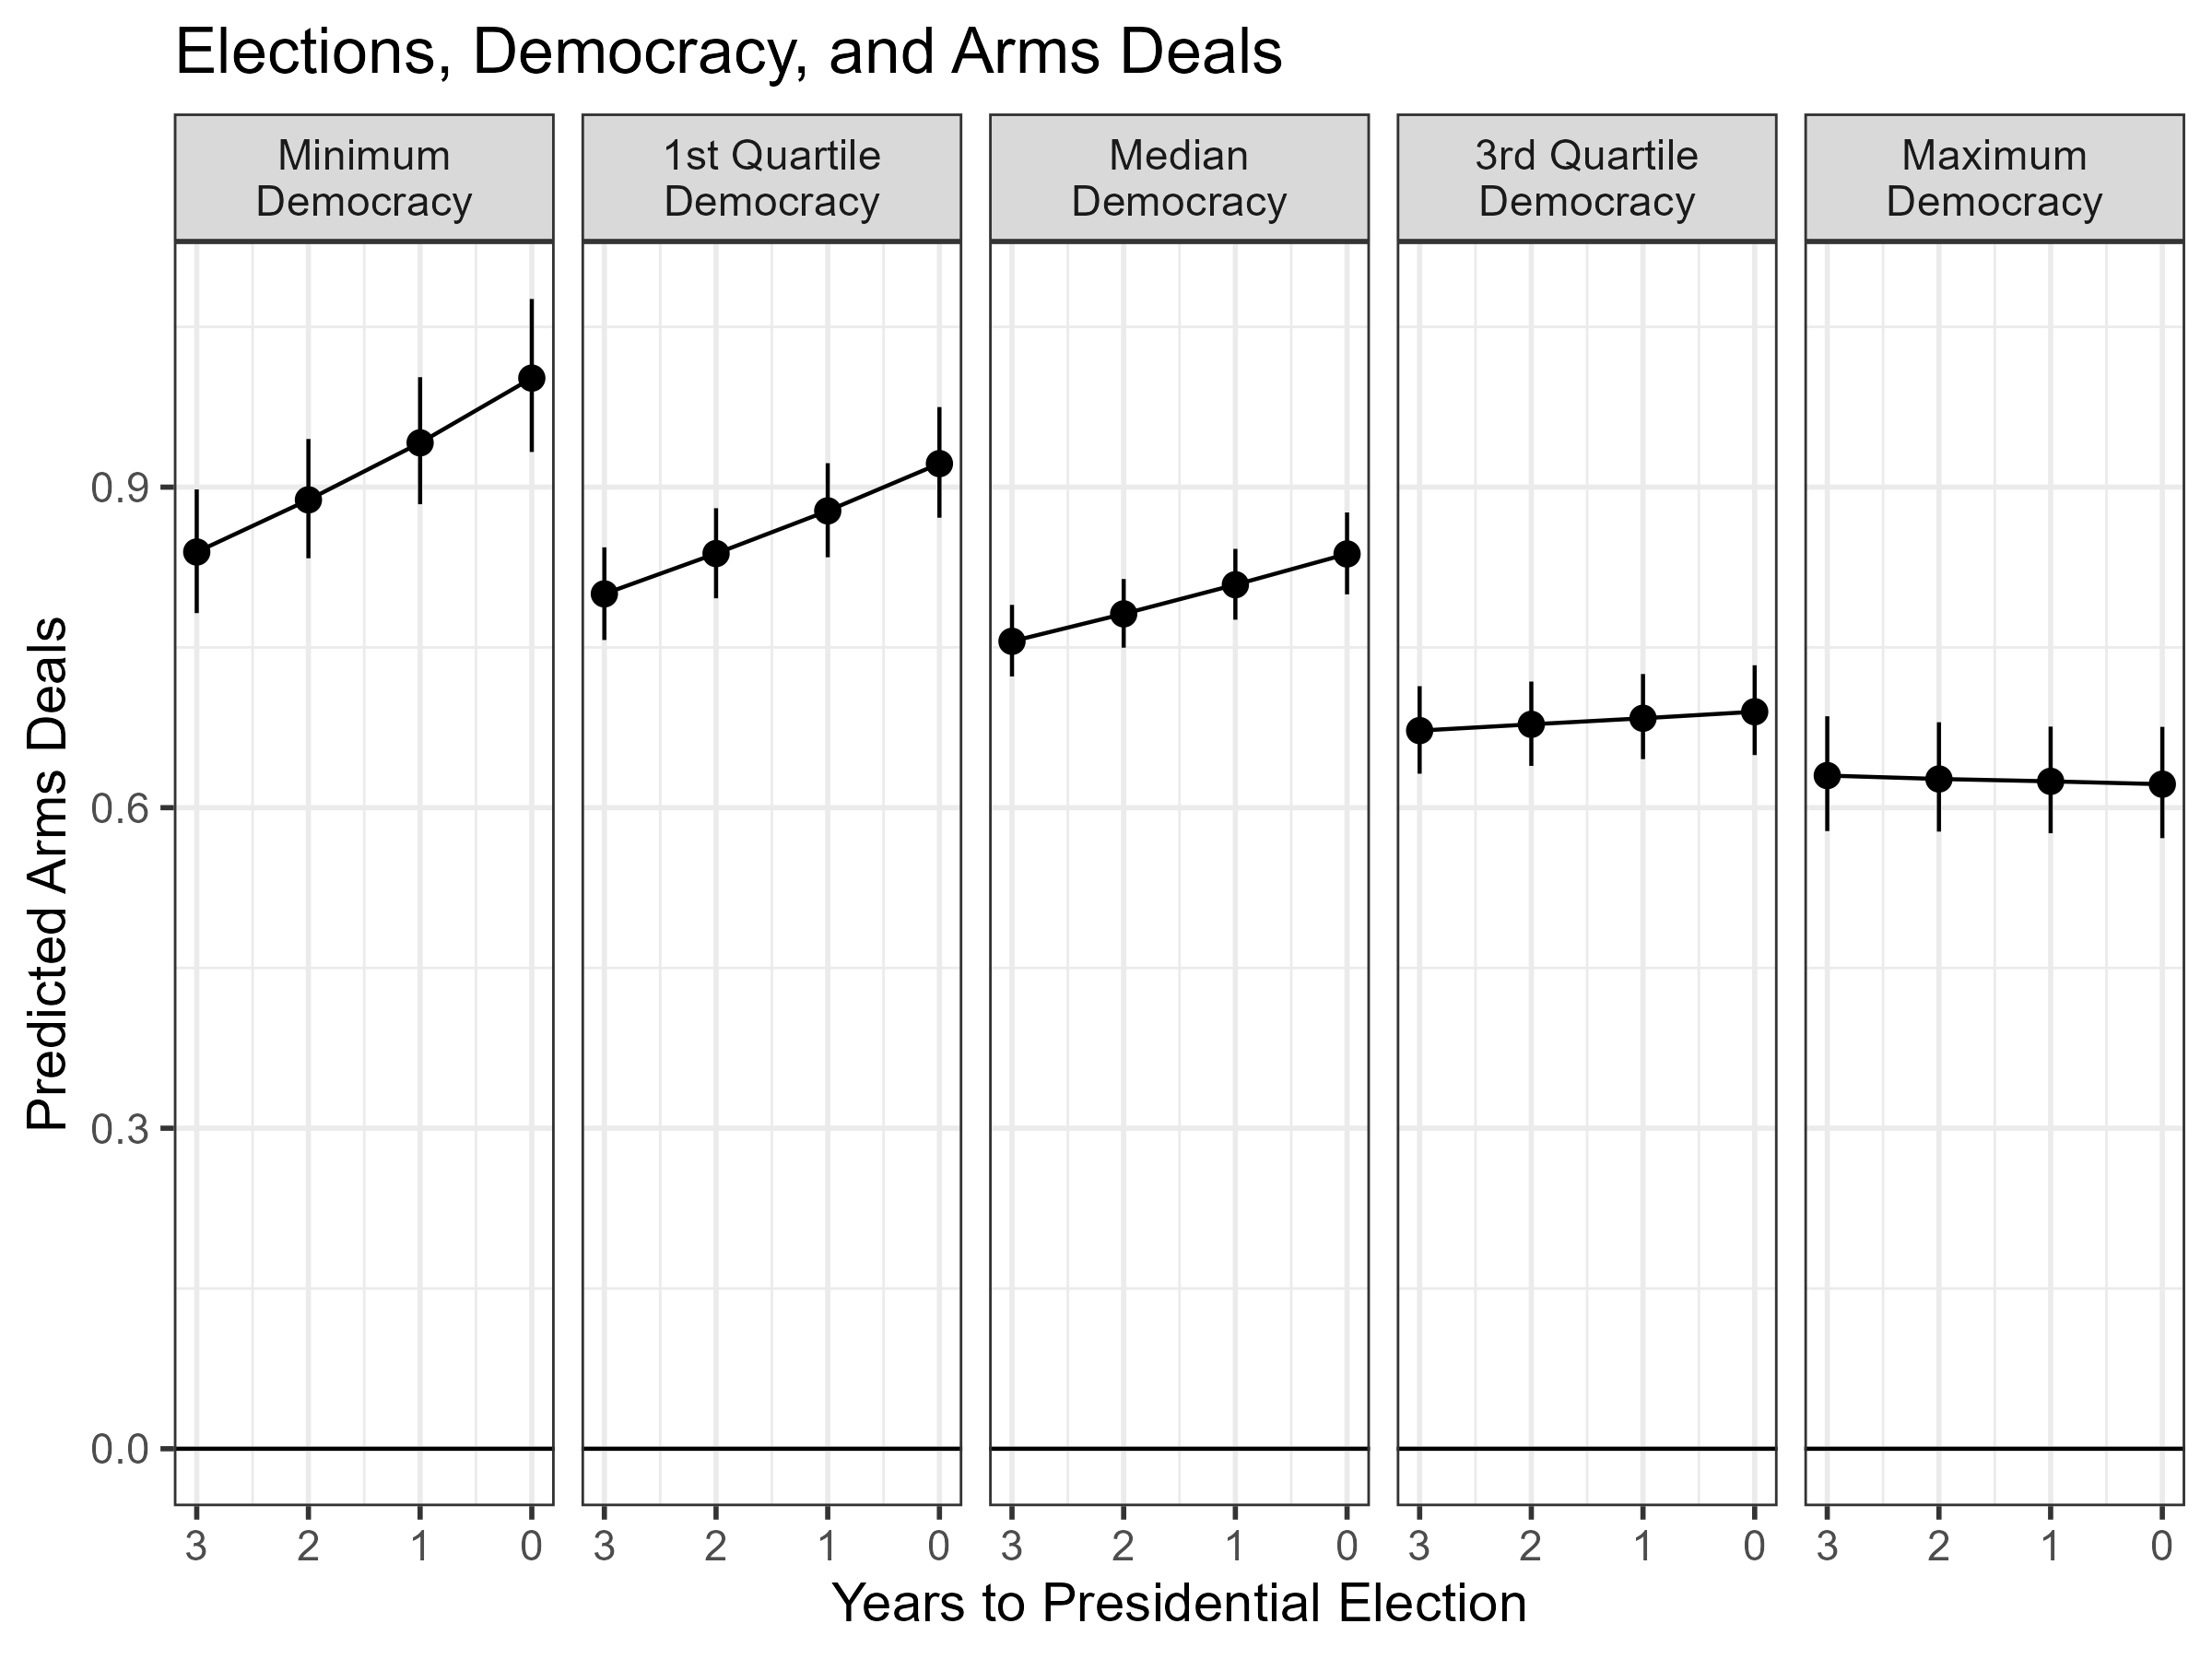
\includegraphics[width=0.95\textwidth]{../figures/democ-deals-pred.png}
	\caption{Predicted arms deals between the United States and other states 1950 to 2014 based on presidential election proximity and partner democracy. Estimates derived from a hurdle Poisson model. Points mark the estimates and error bars summarize the 90\% credible interval.}
	\label{fig:democ-deals-pred}
\end{figure}


\autoref{fig:us-arms-plots} indicates that electoral cycles in arms deals are present for autocracies allies and absent for democracies.
At minimum polyarchy, predicted arms deals rise from .84 to 1 throughout the presidential election cycle.
Hypothesis tests suggest that for a maximally autocratic state, the increase of .06 deals in each year of the electoral cycle is is clearly positive.\footnote{The entire posterior mass of the difference between three and zero years to an election is positive, with a 95\% credible interval that ranges from .1 to .22.}
Electoral cycles when democracy is at the 1st quartile or median are smaller but clearly positive.
The arms deal cycle diminishes as democracy increases, so states with a polyarchy score from the third quartile on see no change in arms deals as elections approach.\footnote{I show in the appendix that these estimates and the interaction between swing states and deals in the next section are robust to using binning estimators.}  


Furthermore, predicted arms deal levels increase as polyarchy decreases. 
This further supports expectations that autocracies are more willing and able to make arms deals that democracies. 
At a minimum, autocracies have fewer political constraints. 


As presidential elections approach, arms deals with autocracies rise. 
The deals and contracts hypothesis predicts that greater arms deals increase defense contracting in swing states. 
The next analysis examines the deals and contracts connection.


\section{Arms Deals and Defense Contracting}


% describe the model 
Linking arms deals and defense contracting is challenging. 
Deals occur between countries, while defense contracting for electoral advantage takes place within U.S. states.
While jointly modeling deals and contracts is theoretically possible, summing country-year deal estimates into an annual measure of total deals for the state-level analysis creates an aggregation problem. %\footnote{A time-series model of aggregate defense deals could address this problem, but it would not show regime differences in arms deals.}
To maintain simplicity, this analysis uses observed annual deals, electoral competition and state-level factors to predict defense contract awards from 2001 to 2020. 


I draw the outcome measure from Department of Defense prime contract award data in the USAspending.gov database.\footnote{Link here: \url{https://www.usaspending.gov/download_center/custom_award_data}.} 
This archive contains individual contracts from 2000 to 2020.\footnote{I analyze defense contracting in these years because archive starts in the 2000 fiscal year and some state-level controls have limited coverage after 2020.}
Although other contracting datasets have longer temporal coverage, they contain less information.
I use the individual contracts data because it allows me to examine the role of electoral geography, and later to link arms deals and contracts in defense industry sectors. 


The key outcome is total defense contracts awarded to each state every year, measured in millions of U.S. dollars.
I focus on contracts for arms production, because arms deals should have little impact on contracts for other goods like construction equipment or food.
While connecting individual contracts and foreign military sales is challenging, the narrow focus on arms production and subsequent analysis matching deals cycles and contracts across defense industrial sectors mean that this approach still provides a useful test. 


Total defense contracts are challenging to model, because some states have no weapons contract awards in a given year, and other states receive billions of dollars in contracts. 
The resulting outcome is zero-valued and right-skewed. 
Transformations of such data can make substantive effect calculations challenging and potentially biased. 
Traditional approaches such as logging the outcome after adding one are sensitive to the outcome scale and the constant added \citep{ChenRoth2022, MullahyNorton2022}. 


To overcome these issues, I fit two types of models.
First, I rescale the defense contracts measure to fall between zero and one by expressing each state's contracts as a share of total defense contracting in that year.
I then use ordered beta regression to predict the rescaled outcome \citep{Kubinec2022}.\footnote{\url{https://www.robertkubinec.com/post/logs/}} 
This allows me to use a flexible outcome distribution, account for zeros and avoid scale-effects from log-transformations and working with outcomes in millions of dollars. 
Converting the coefficients and marginal effects back to the outcome scale after estimation is straightforward, as I multiply the model estimates by the rescaling constant.
I also fit a a hurdle lognormal model of contracts without any transformation and a robust regression of annual contract changes. 
Both approaches give similar inferences.\footnote{See the appendix for results.} 


The first independent variable is total annual arms deals.  
I measure arms deals by summing U.S. arms deals with all countries in every year. 
Annual deals range from 75 to 160. 
Next, I include a dummy indicator of swing state status based on \citet{KrinerReeves2015}.
Swing states are states where the losing party won at least 45\% of the two-party vote in three straight elections. 


I then interact the swing state dummy with total U.S. arms deals. 
My argument expects that the constituent term of arms deals, which expresses the association between deals and contracts outside of swing states, should be negligible or negative.
Because there are no years with zero U.S. arms deals, the swing state constituent term is not directly meaningful.  
The interaction term for swing states and annual deals should be positive.


In addition to the electoral competition and deals variables, I include several controls. 
First, I adjust for population and GDP, because larger and more prosperous states receive more contracts. 
Other electoral competition indicators include the time to a presidential election and whether a state is a core member of the president's coalition \citep{KrinerReeves2015}. 
I also control for increased defense contracting demand during peak years in the global war on terror with a dummy variable that is equal to one from 2001 to 2011. 
The final control adjusts for presidential partisanship by dummy coding Republican presidencies. 


Further adjustments in the model account for the data structure.
First, I include state varying intercepts because observations cluster within states. 
Current contracting also depends on past contracting, but this varies across divergent state defense industries. 
I therefore include a state-specific lagged dependent variable, which allows temporal dependence in contracting to vary by state.\footnote{See the appendix for state parameter estimates.}


%Formally, the state-level equation is: 
%\begin{equation}
%\mu_{st}^{cont} = \alpha_{state} + \theta_s y_{st-1} + \rho_1 \mbox{Deals} + \rho_2 \mbox{Swing} + \rho_3 \mbox{Deals} * \mbox{Swing} + \textbf{G} \lambda
%\end{equation}


%This model is a useful test of the second hypothesis, as it assesses the impact of arms deals on swing states while adjusting for clustering, temporal variation and other predictors.
%The next section summarizes the estimates. 


\subsection{Results}


Because one of the interaction coefficients has no substantive meaning, I focus on marginal effects and predicted outcomes.
In \autoref{fig:deals-swing-me}, I present the impact of deals, swing state competition, and predicted outcomes.
All these estimates suggest that deals increase defense contracting awards to swing states. 
To test the deals and contracts hypothesis, I examine the positive posterior mass of the interaction between arms deals and swing states, because the hypothesis expects a positive association.\footnote{For the marginal effect of swing status and outcome predictions, I again use 90\% credible intervals, because they are less sensitive to simulation variance.}


First, the impact of increasing arms deals on defense contracting is unclear outside of swing states, but clearly positive in swing states. 
Only 34\% of the posterior mass in the deals constituent term is positive, so there is little evidence that deals increase contract awards outside of swing states. 
98\% of the posterior mass of the deals and swing state interaction is positive, however. 
The preponderance of evidence supports the deals and contracts hypothesis.


\begin{figure}[htpb]
	\centering
		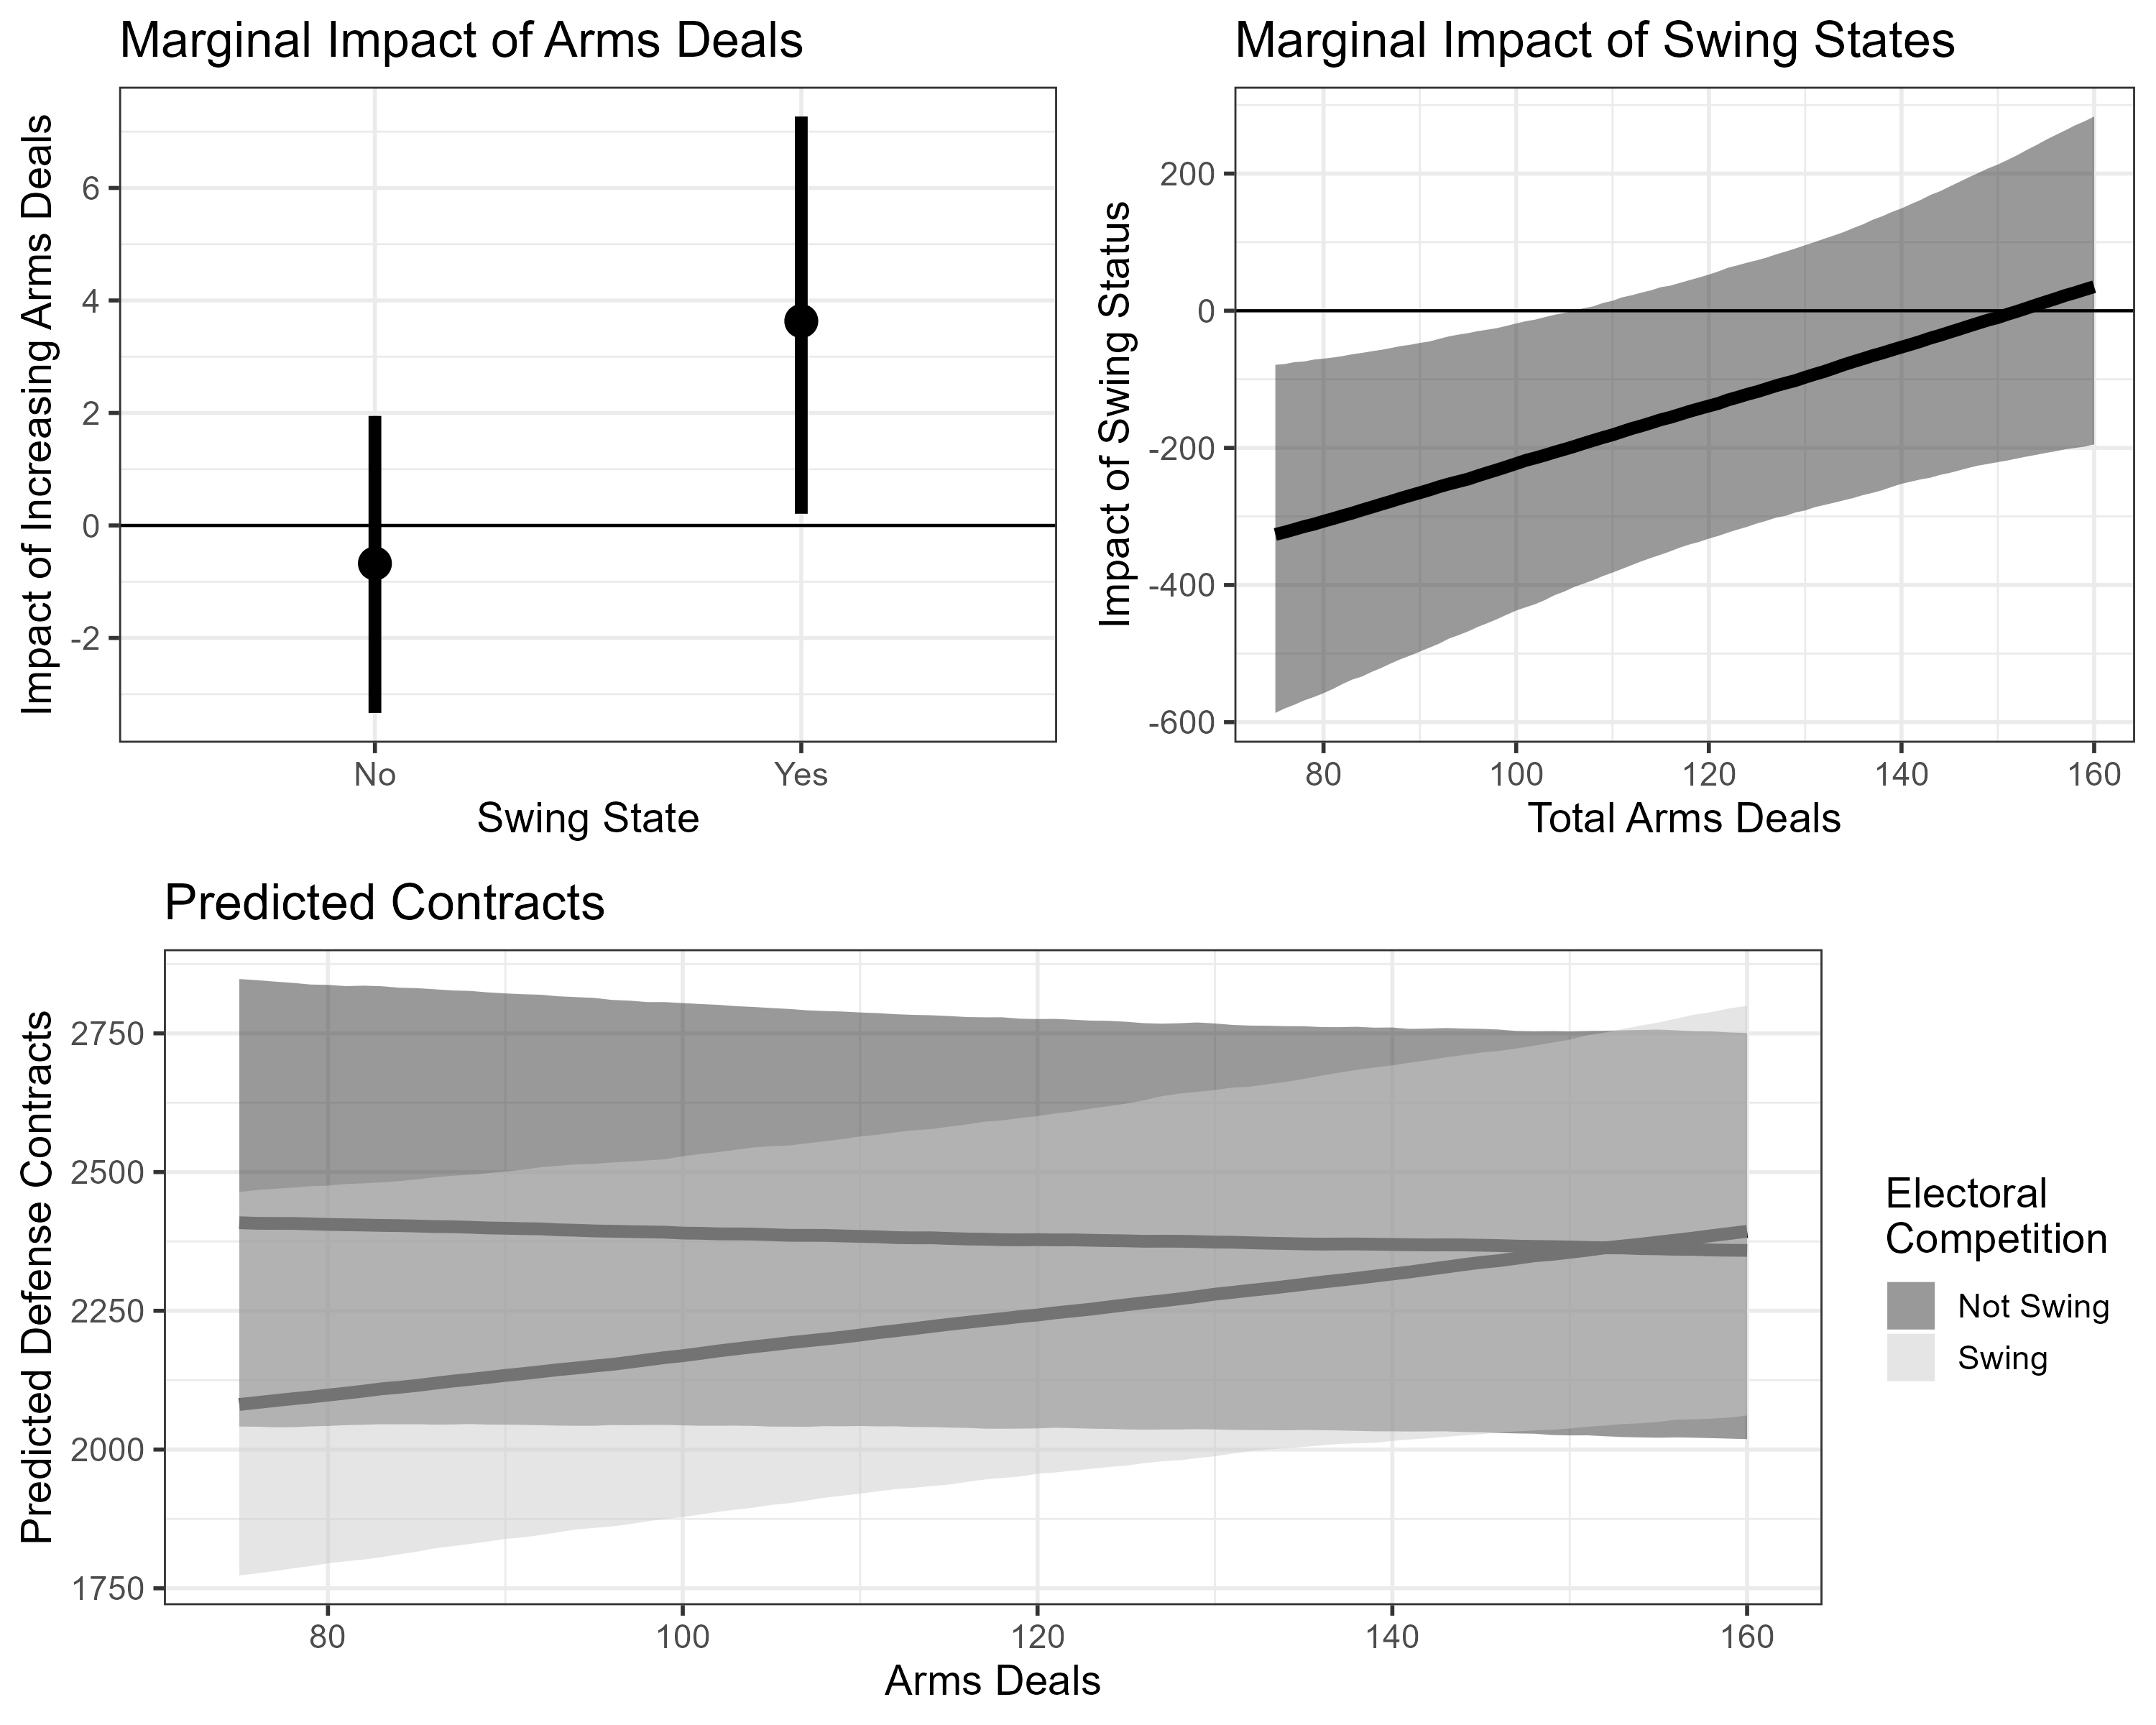
\includegraphics[width=0.95\textwidth]{../figures/deals-swing-me.png}
	\caption{Interaction coefficients, marginal effects and predicted outcomes from an interaction of swing state status and U.S. arms deals. The outcome is annual defense contracts in the 50 U.S. states from 2001 to 2020, measured in millions of dollars. Lines give the expected value, while the error bars summarize 90\% credible intervals. All other variables fixed at the mode or median.}
	\label{fig:deals-swing-me}
\end{figure}


The coefficient estimates in \autoref{fig:deals-swing-me} imply that moving from the first to the third quartile of deals increases defense contracting by \$202 million in a swing state, all else equal. 
Greater deals are less connected to contract awards outside swing states because the share of contracts that go to swing states rises in election years. 
Leaders thus use arms deals to target critical constituencies.


Second, swing states receive more defense contracts as arms deals rise. 
At the observed minimum of arms deals, a typical swing state receives \$2.5 billion less in contracts.
The initial swing state disadvantage occurs because non-swing states like California and Texas have substantial defense industries.
When arms deals approach the observed maximum, swing states receive similar contracts to other states. 


Finally, predicted defense contracts increase as arms deals increase, but only in swing states, as the bottom panel of \autoref{fig:deals-swing-me} shows. 
Holding all else equal, increasing arms deals leads to greater contracts in swing states. 
Defense contracts in non-swing states do not respond to increasing arms deals.
As a result, the gap in defense contracting between swing and other states disappears in years with high arms deals. 



These estimates support the deals and defense contracts hypothesis. 
Increasing arms deals are correlated with greater defense contracts in swing states. 
As a result, swing states receive similar contracts to other states with larger economies and less electoral competition. 



%Next, I use these estimates and the model of arms deals to estimate how much electoral cycles in arms deals with U.S. allies add to defense contracting levels in swing states.  
%
%
%\subsection{Calculating the Defense Contracting Consequences of Arms Deals with Autocratic Allies}
%
%
%The following calculation is necessarily rough, as I combine predictions from two separate models. 
%To give a sense of how much defense contracting in swing states is due to arms deal cycles, I use predictions from hypothetical and observed data.
%Both these suggest that the increases in arms deals captured in \autoref{fig:us-arms-plots} are a substantively meaningful contributor to defense contracting in swing states. 

%
%Given these marginal effects, calculating the partial impact of alliances and allied regimes on deals and ultimately contracts is straightforward. 
%Across the electoral cycle with eight hypothetical countries of varying democracy and alliance status in \autoref{fig:democ-deals-pred}, there is one more arms deal in the election year, compared to the year after an election. 
%The marginal effect of arms deals is \$3.6 million, so the hypothetical cycle in deals and contracts adds several million in defense contracting to one swing state. 
%%
%
%These partial equilibrium associations are simple, but they may somewhat understate the impact of arms deals. 
%Because almost all defense production of finished and intermediate goods spans the United States, arms deals affect multiple swing states. 
%I therefore use predictions from observed data to assess the substantive impact of increasing arms deals. 


\section{Examining the Theoretical Process}


The results so far corroborate two predictions of the argument, but require additional validation. 
In the following, I check the low constraint and high security motivation mechanisms by showing that allies drive most of the electoral cycle in U.S. arms deals with autocracies.  
Given a strong security motivation to make arms deals, autocratic allies have the necessary mix of means and motivation to make arms deals.


After examining the role of alliances in arms deals cycles, I establish that the same platforms in arms deals between the United States and autocratic allies are also strongly correlated with swing state contracts.
If the platforms that moved in deals cycles were uncorrelated with swing state contracts, that would suggest any connection between deal cycles and swing state contracts is coincidental.
The sectoral consistency I find instead suggests that arms deals do translate into swing state contracts.\footnote{A third process check in the appendix shows that the marginal impact of arms deals on swing state contracts is positive in the year before and year of a presidential election and is closer to zero otherwise.}



\subsection{Autocratic Allies}


% mechanisms
The argument claims that autocracies make arms deals with the United States near elections because their leaders have fewer constraints and reap security benefits. 
The confluence of security need and freedom to make deals is necessary for cycles. 
Autocratic allies of the United States have equal political flexibility and greater security motivation than other autocrats. 
As a result, allied states should drive most of the electoral cycle in autocratic arms deals.


% potential markets: allies
% take new or used stuff to make room
Alliances increase arms transfers in general. 
\citet{Thurneretal2019} find that while the importance of security and economic factors fluctuates, alliances consistently increase arms transfers.
%Common security interests and defense industrial cooperation create economic and security ties that encourage arms trade \citep{Bitzinger1994}. 
\citet[pg. 184-5]{IkenberryGrieco2003} note that states often use direct transfers to attract and sustain security commitments. 
U.S. allies that rely on American weapons, systems and doctrines can also integrate purchases more easily and build on past orders. 


% security need
Autocratic allies also have additional security motivation to facilitate electoral arms deal cycles. 
Deals that win favor with U.S. leaders increase the odds of U.S. support for a partner's foreign policy goals and political survival.  
In addition to the capability boost of new arms, allies gain confidence in U.S. commitment because arms exports are a costly signal \citep{McManusYarhi-Milo2017}, and U.S. leaders rely on arms to support autocratic partners \citep{Yarhi-Miloetal2016}.


% less export cycles to non-allies
% each evidence sentence could be its own paragraph 
Furthermore, the security externalities of arms transfers reduce electoral cycles in arms exports to non-allies. 
U.S. leaders will be less willing to increase the capability of states with fewer common interests, even if it facilitates contracting cycles.
Justifying deals is still challenging, but it is more straightforward for autocratic allies. 



%Other U.S. elites are also more likely to object to arms deals outside alliances.
%Leaders could suffer electoral costs if other elites publicly criticize deals \citep{Saunders2022}.
%Arms transfers to non-allies could face greater opposition scrutiny near elections, leading presidents to forestall criticism by forgoing contentious transfers.
%Limited defense industry cooperation further constrains exports outside alliances, while allies with defense industrial ties can receive intermediate goods as well.


% Sales and transfers- who pays for what
%Moreover, prot{\'e}g{\'e}s do not always pay for U.S. arms.
%The United States often subsidizes or gifts arms transfers through foreign military sales programs. 
%While these still count as arms exports, they impose few immediate costs on recipients.
%Alliances make such subsidized transfers easier to justify to other elites, as they promote common security interests. 


% sum it up
Among autocracies, U.S. allies mix stronger security motivations with the same low constraints. 
Autocratic allies thus have the necessary means and motivation to buy arms near elections. 
Alliances also make it easier for U.S. leaders to justify deals.
As a result, most of the electoral cycle in arms deals with autocracies should occur with allied states. 
 

 
\subsubsection{Results}

I tweak the hurdle Poisson model of autocracies and electoral arms deals to examine the role of alliances. 
To do this, I add a dummy indicator of whether a state is a U.S. ally to the interaction of partner regime and presidential election proximity.\footnote{This includes formal and informal allies.}
This creates a triple interaction of alliance, regime type, and election timing. 


Because interpreting coefficients in triple interactions is challenging, I summarize the interaction of alliances, democracy and presidential election proximity in \autoref{fig:us-arms-plots}.
This figure plots predicted arms deals based on proximity to a presidential election, democracy and alliance status. 
Each facet divides estimates based on democracy, while colors distinguish between allied and non-allied states. 


\begin{figure}[htpb]
	\centering
		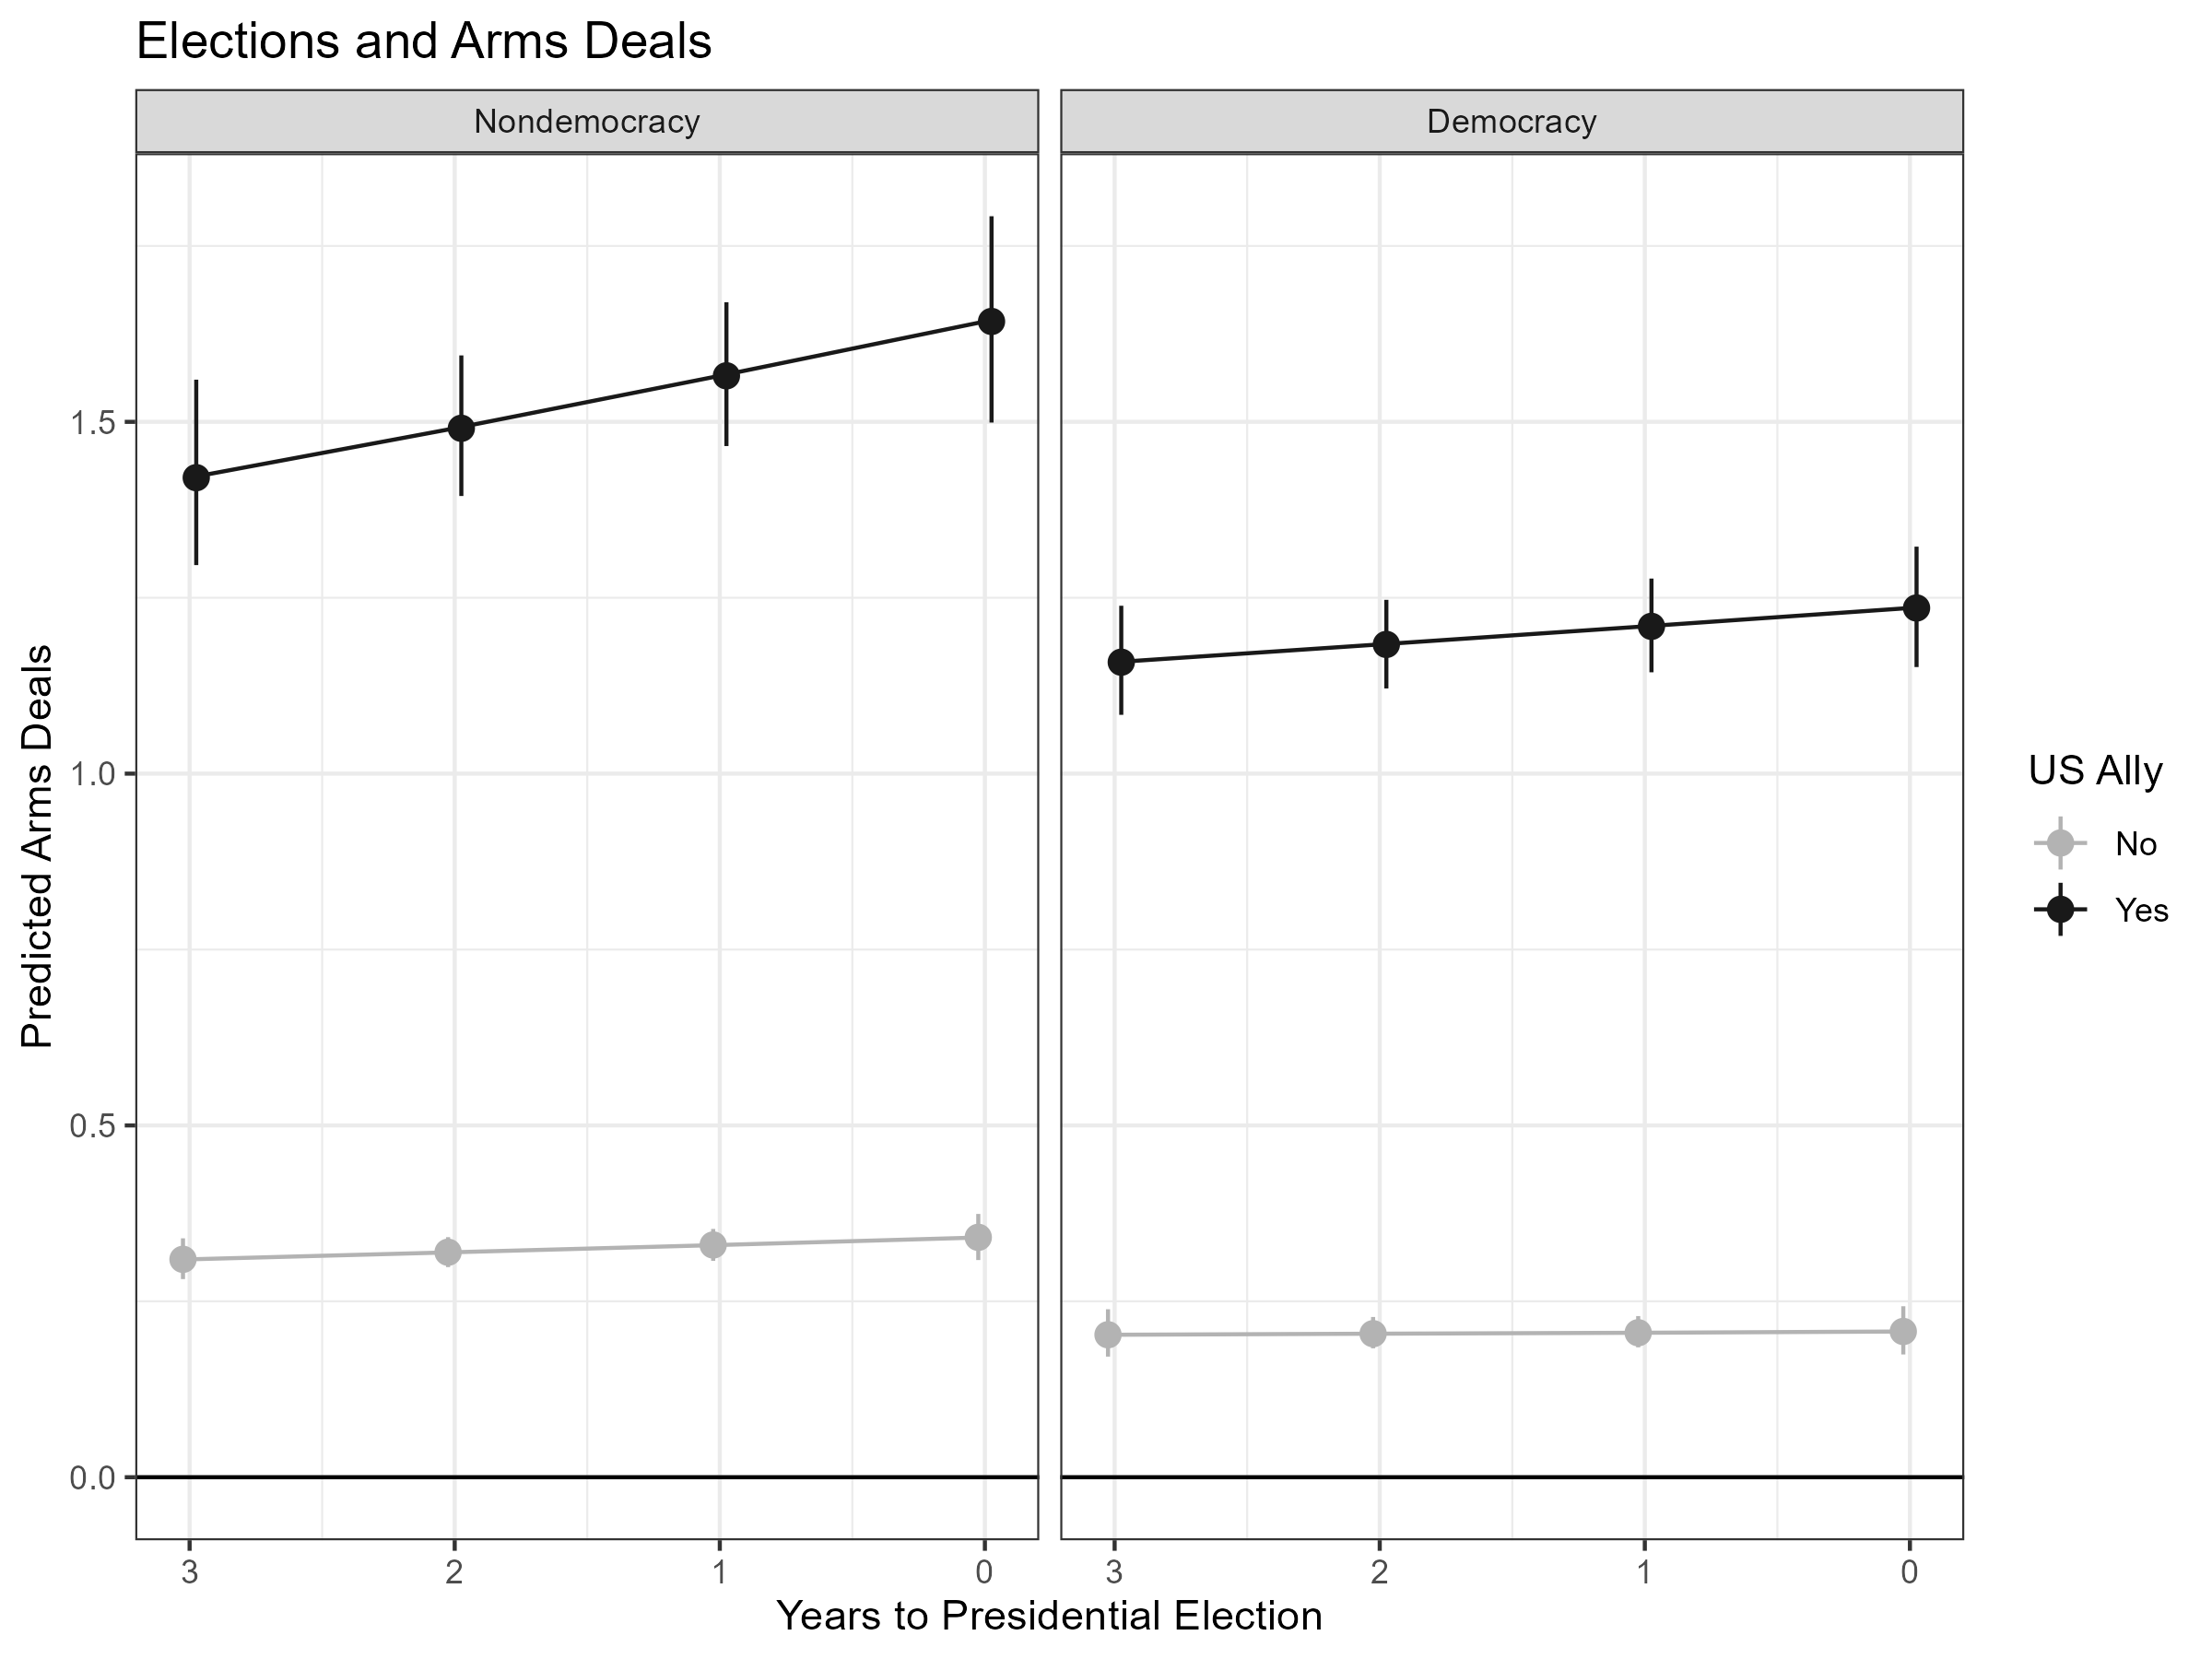
\includegraphics[width=0.95\textwidth]{../figures/us-arms-plots.png}
	\caption{Predicted arms deals between the United States and other states 1950 to 2014 based on presidential election proximity, democracy, and security alliances. Estimates derived from a hurdle Poisson model. Points mark the estimates and error bars summarize the 90\% credible interval. All other variables fixed to their mode or median.}
	\label{fig:us-arms-plots}
\end{figure}


The estimates in \autoref{fig:us-arms-plots} suggest that allies are responsible for most of the electoral cycle in U.S. arms deals with autocracies. 
The United States makes more arms deals with allied states than non-allied states, regardless of partner regime. 
Predicted deals with non-allied states are lower regardless of democracy. 


There are cycles in arms deals for autocracies with and without a U.S. alliance, but the cycles are much larger for allied states. 
When allied polyarchy is at the minimum, predicted arms deals rise from 2.3 to 2.7 throughout the presidential election cycle.
Hypothesis tests of equality between allied arms deals at minimum democracy indicate a clear increase of .13 deals in each year of the electoral cycle.\footnote{The 95\% credible interval ranges from .05 to .21.}
Non-allied states with a minimal polyarchy score see predicted deals increase by roughly .05 a year.


Unlike autocratic allies, democratic allies receive consistent arms deals. 
Defense industrial integration may explain some of the democratic stability \citep{Brooks2005}, but another plausible explanation is that democratic leaders face more constraints on making deals around presidential elections.
The constraint argument is also plausible because democracies make fewer arms deals overall. 


Electoral cycles in arms deals are strongest for autocratic allies. 
Alliances increase the level of arms deals, and autocracies respond more to presidential elections. 
This suggests that autocracies with both political flexibility and security motivation make arms deals that ultimately feed swing state contracts. 
In the next section, I use specific defense industrial sectors to check that connection between deals and contracts. 



\subsection{Which Weapons Drive Deals and Contracts?} 


The final analysis examines whether the weapons systems that change hands in U.S. arms deals with autocratic allies and are correlated with swing-state contract awards. 
Showing that the United States makes more deals for specific weapons as elections approach, and that deals for those weapons correlate with defense contract awards in swing states increases confidence in the theoretical process.\footnote{These correlations do not link specific deals and contracts, however.}
I find that aircraft are the most common subject of arms deals with autocrats near elections, and aircraft deals also increase swing state contracts for aircraft production.


To analyze deals by sector, I divided arms deals and defense contracts into six sectors. 
The sectors include aircraft, arms and munitions, military electronics, missiles and space technology, ships, and vehicles.  
Each of these sectors has a distinct production geography and arms deal distribution.


I then fit six hurdle Poisson models, one for each type of arms deals. 
These models use the same covariates as the preceding arms deals model; a triple interaction of alliance, democracy and election timing, along with a series of controls and a hurdle equation.
Using the hurdle again improves model fit, as more country-year observations have zero deals within sectors. 


For ease of presentation, I plot predicted arms deals at the minimum and maximum of partner democracy in \autoref{fig:deals-sector}.
The estimates suggest that aircraft are the core weapons system in electoral cycles in arms deals with autocratic allies. 
Military alliances strongly increase the likelihood of arms deals for aircraft and regime type determines how much aircraft deals follow presidential election cycles. 
Aircraft deals with autocratic allies are the most common deal overall, and these deals rise as presidential elections approach. 
While aircraft deals with democratic allies are also common, they respond less to election timing. 



\begin{figure}[htpb]
	\centering
		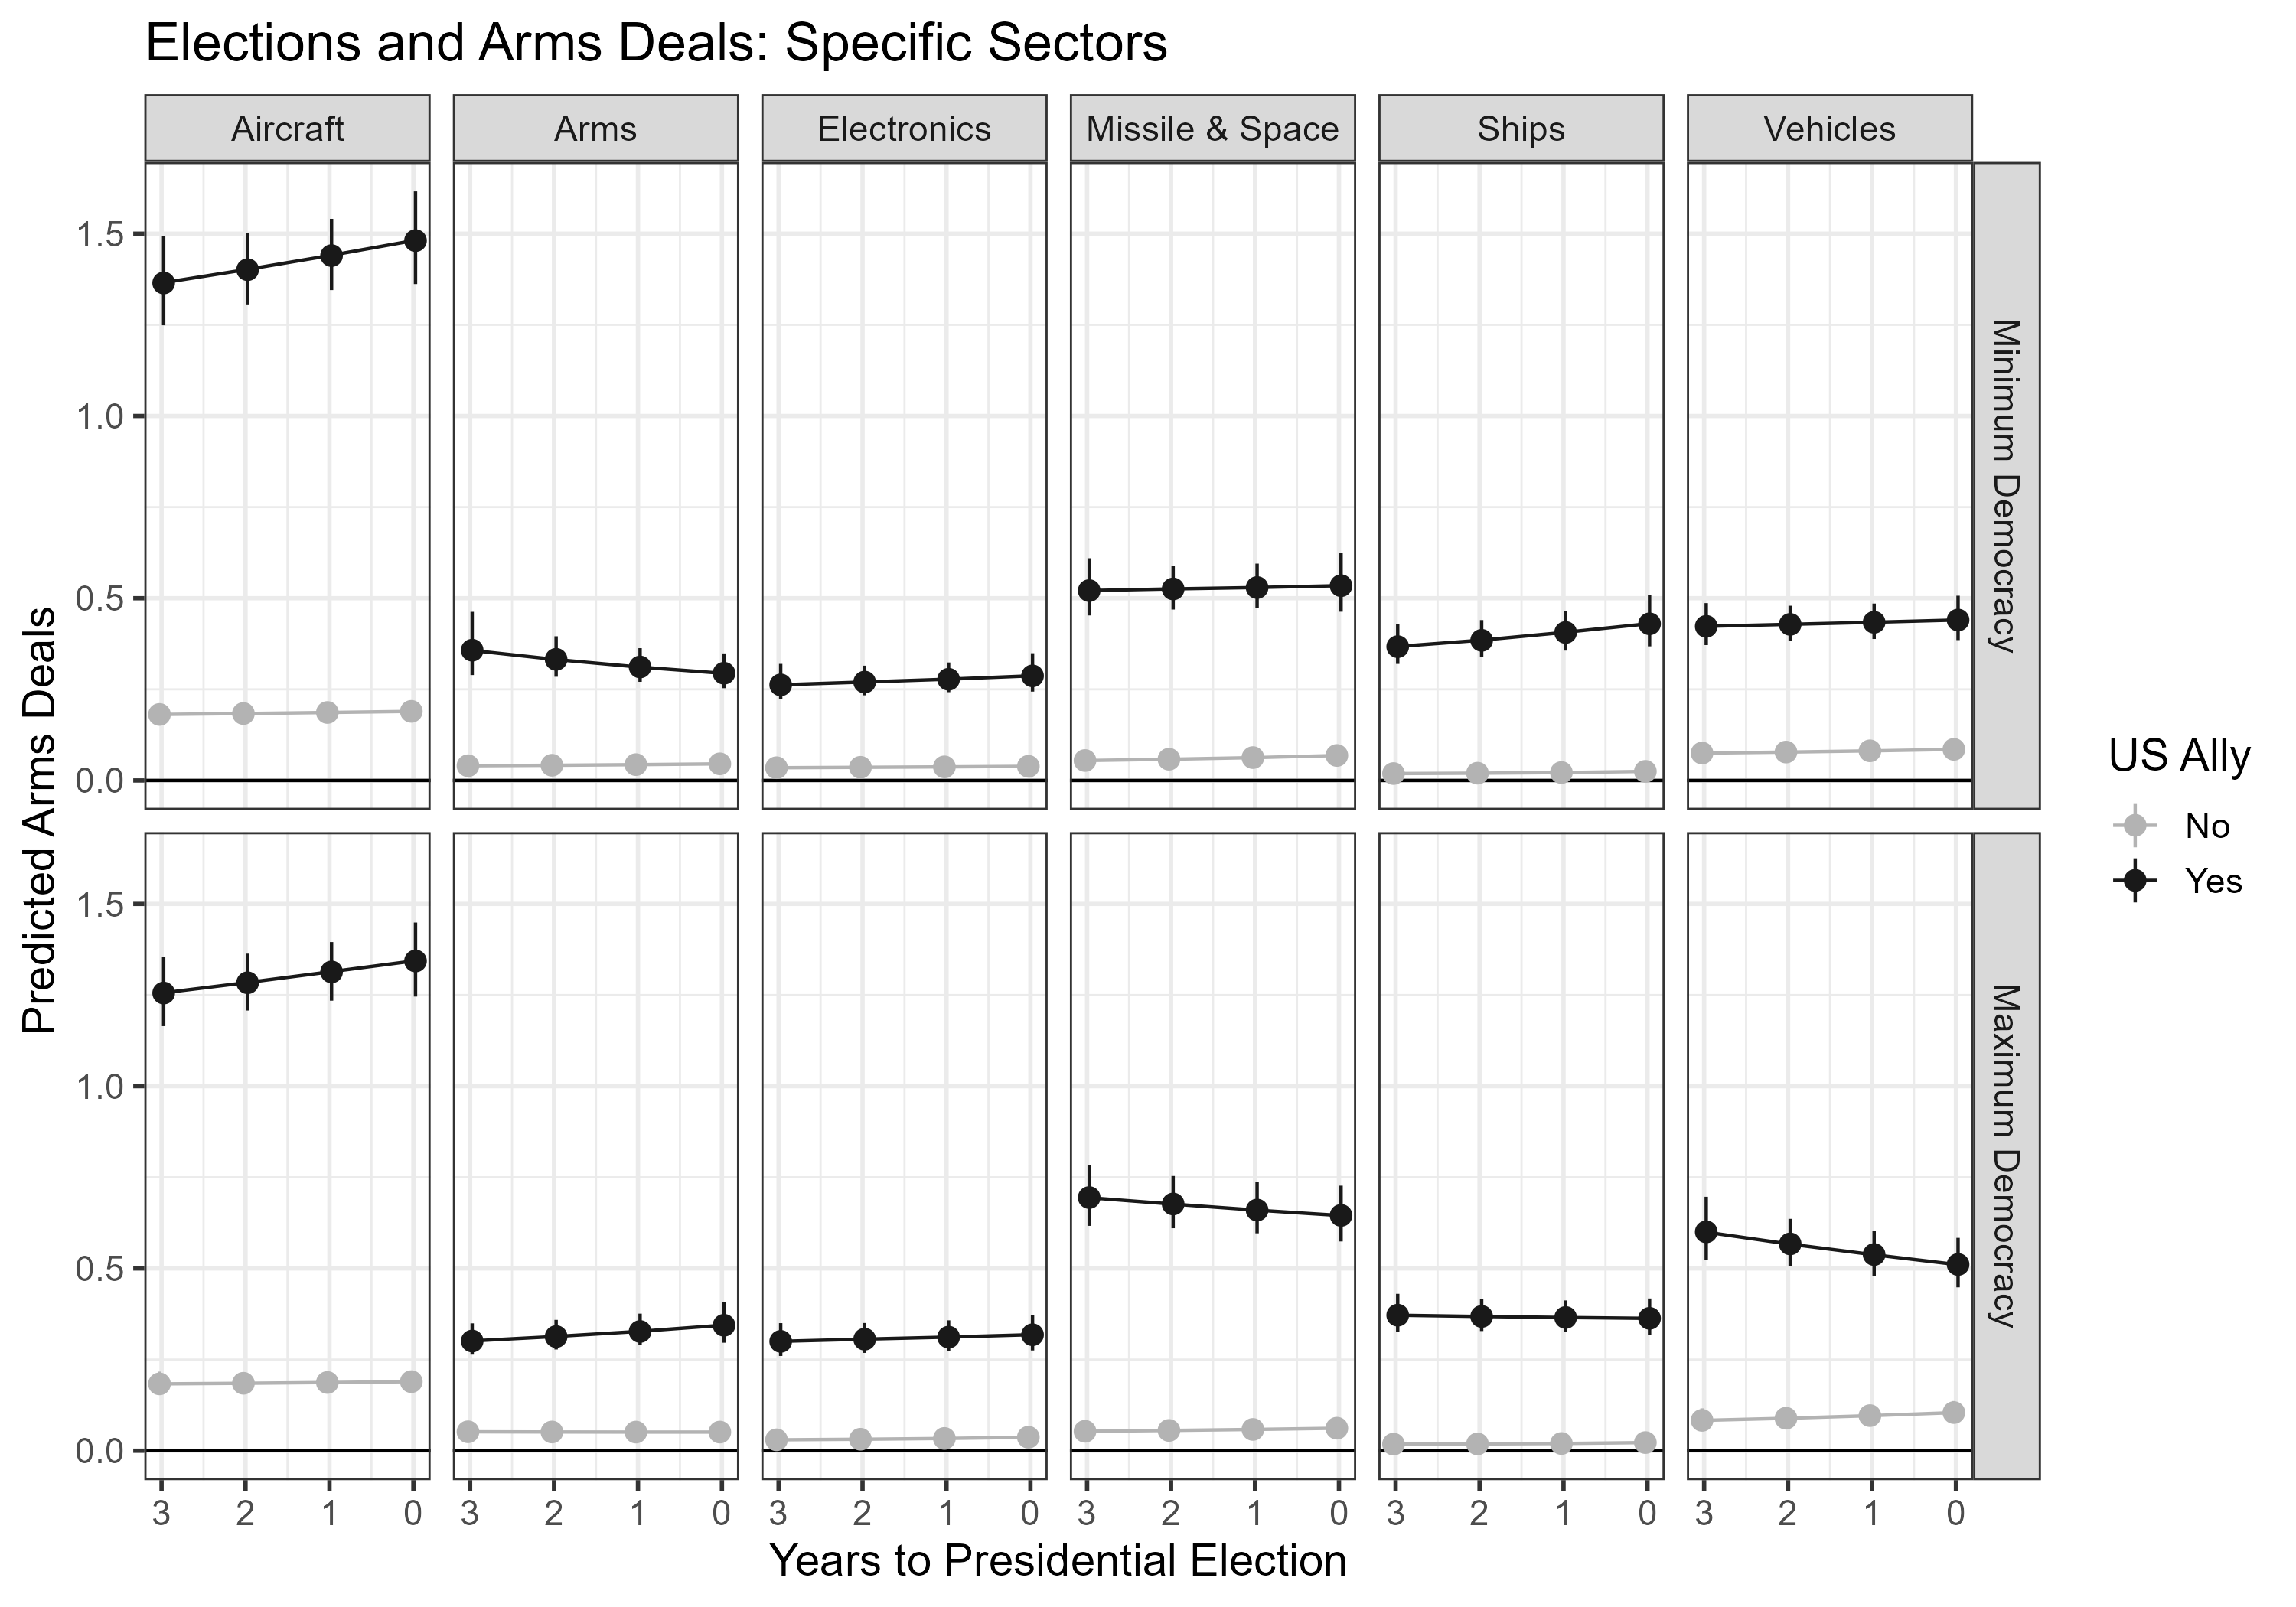
\includegraphics[width=0.95\textwidth]{../figures/deals-sector.png}
	\caption{Predicted arms deals between the United States and other states 1950 to 2020 based on presidential election proximity, democracy, and military alliance. Estimates derived from six sector-specific hurdle Poisson models counting annual deals divided by the type of military good exchanged. Points mark the estimates and error bars summarize the 90\% credible interval. All other variables fixed to their mode or median.}
	\label{fig:deals-sector}
\end{figure}


Among autocracies, alliances increase deals for ships, and ship deals increase with electoral proximity. 
Allies make more ship deals at all levels of democracy, but only autocratic allies make more deals near elections. 
Ships could also move in arms deals that feed defense contracting. 


Other weapons show less evidence of cycles in arms deals. 
Deals for arms and other munitions do not depend on democracy or election timing. 
Democratic allies are more likely to make deals for military electronics and missile/space systems. 
The importance of democracy and alliances for these goods likely reflects joint production and planning in formal U.S. alliances. 


%Neither electronics nor missile and space systems see electoral deal cycles.
%Deals for military vehicles do not track the electoral cycle either. 
%Among autocracies, alliances make no difference for vehicle deals. 
%Allied democracies see small decreases in deals as elections approach. 

\subsubsection{Deals and Defense Contracts by Sector}


Next, I fit six models of defense contracts to examine the deals and contracts hypothesis for each sector and check if the sectors with deal cycles have a clear positive association between deals and swing state contracts. 
This analysis divides total contracts by sector using the product description for each contract. 
As in the analysis of aggregate defense contracting, I rescale the outcome between 0 and 1 using the annual sum of contracts for those defense goods. 
I then fit ordered beta regression models of the rescaled outcomes, using an identical specification to the aggregate defense contracting model.
The key independent variables in these models are observed arms deals in each sector, the binary swing state indicator, and their interaction. 
I also include the same terms to capture state varying intercepts, state-specific autocorrelation, and other controls. 


Aircraft deals are strongly correlated with aircraft contracts in swing states. 
\autoref{fig:me-deals-sector} plots the interaction between different deal types and swing state status.  
These estimates show the deals coefficients from six ordered beta models, transformed back to the outcome scale. 
Again, I focus on the positive posterior mass, as this gives the evidence consistent with a directional hypothesis.


\begin{figure}[htpb]
	\centering
		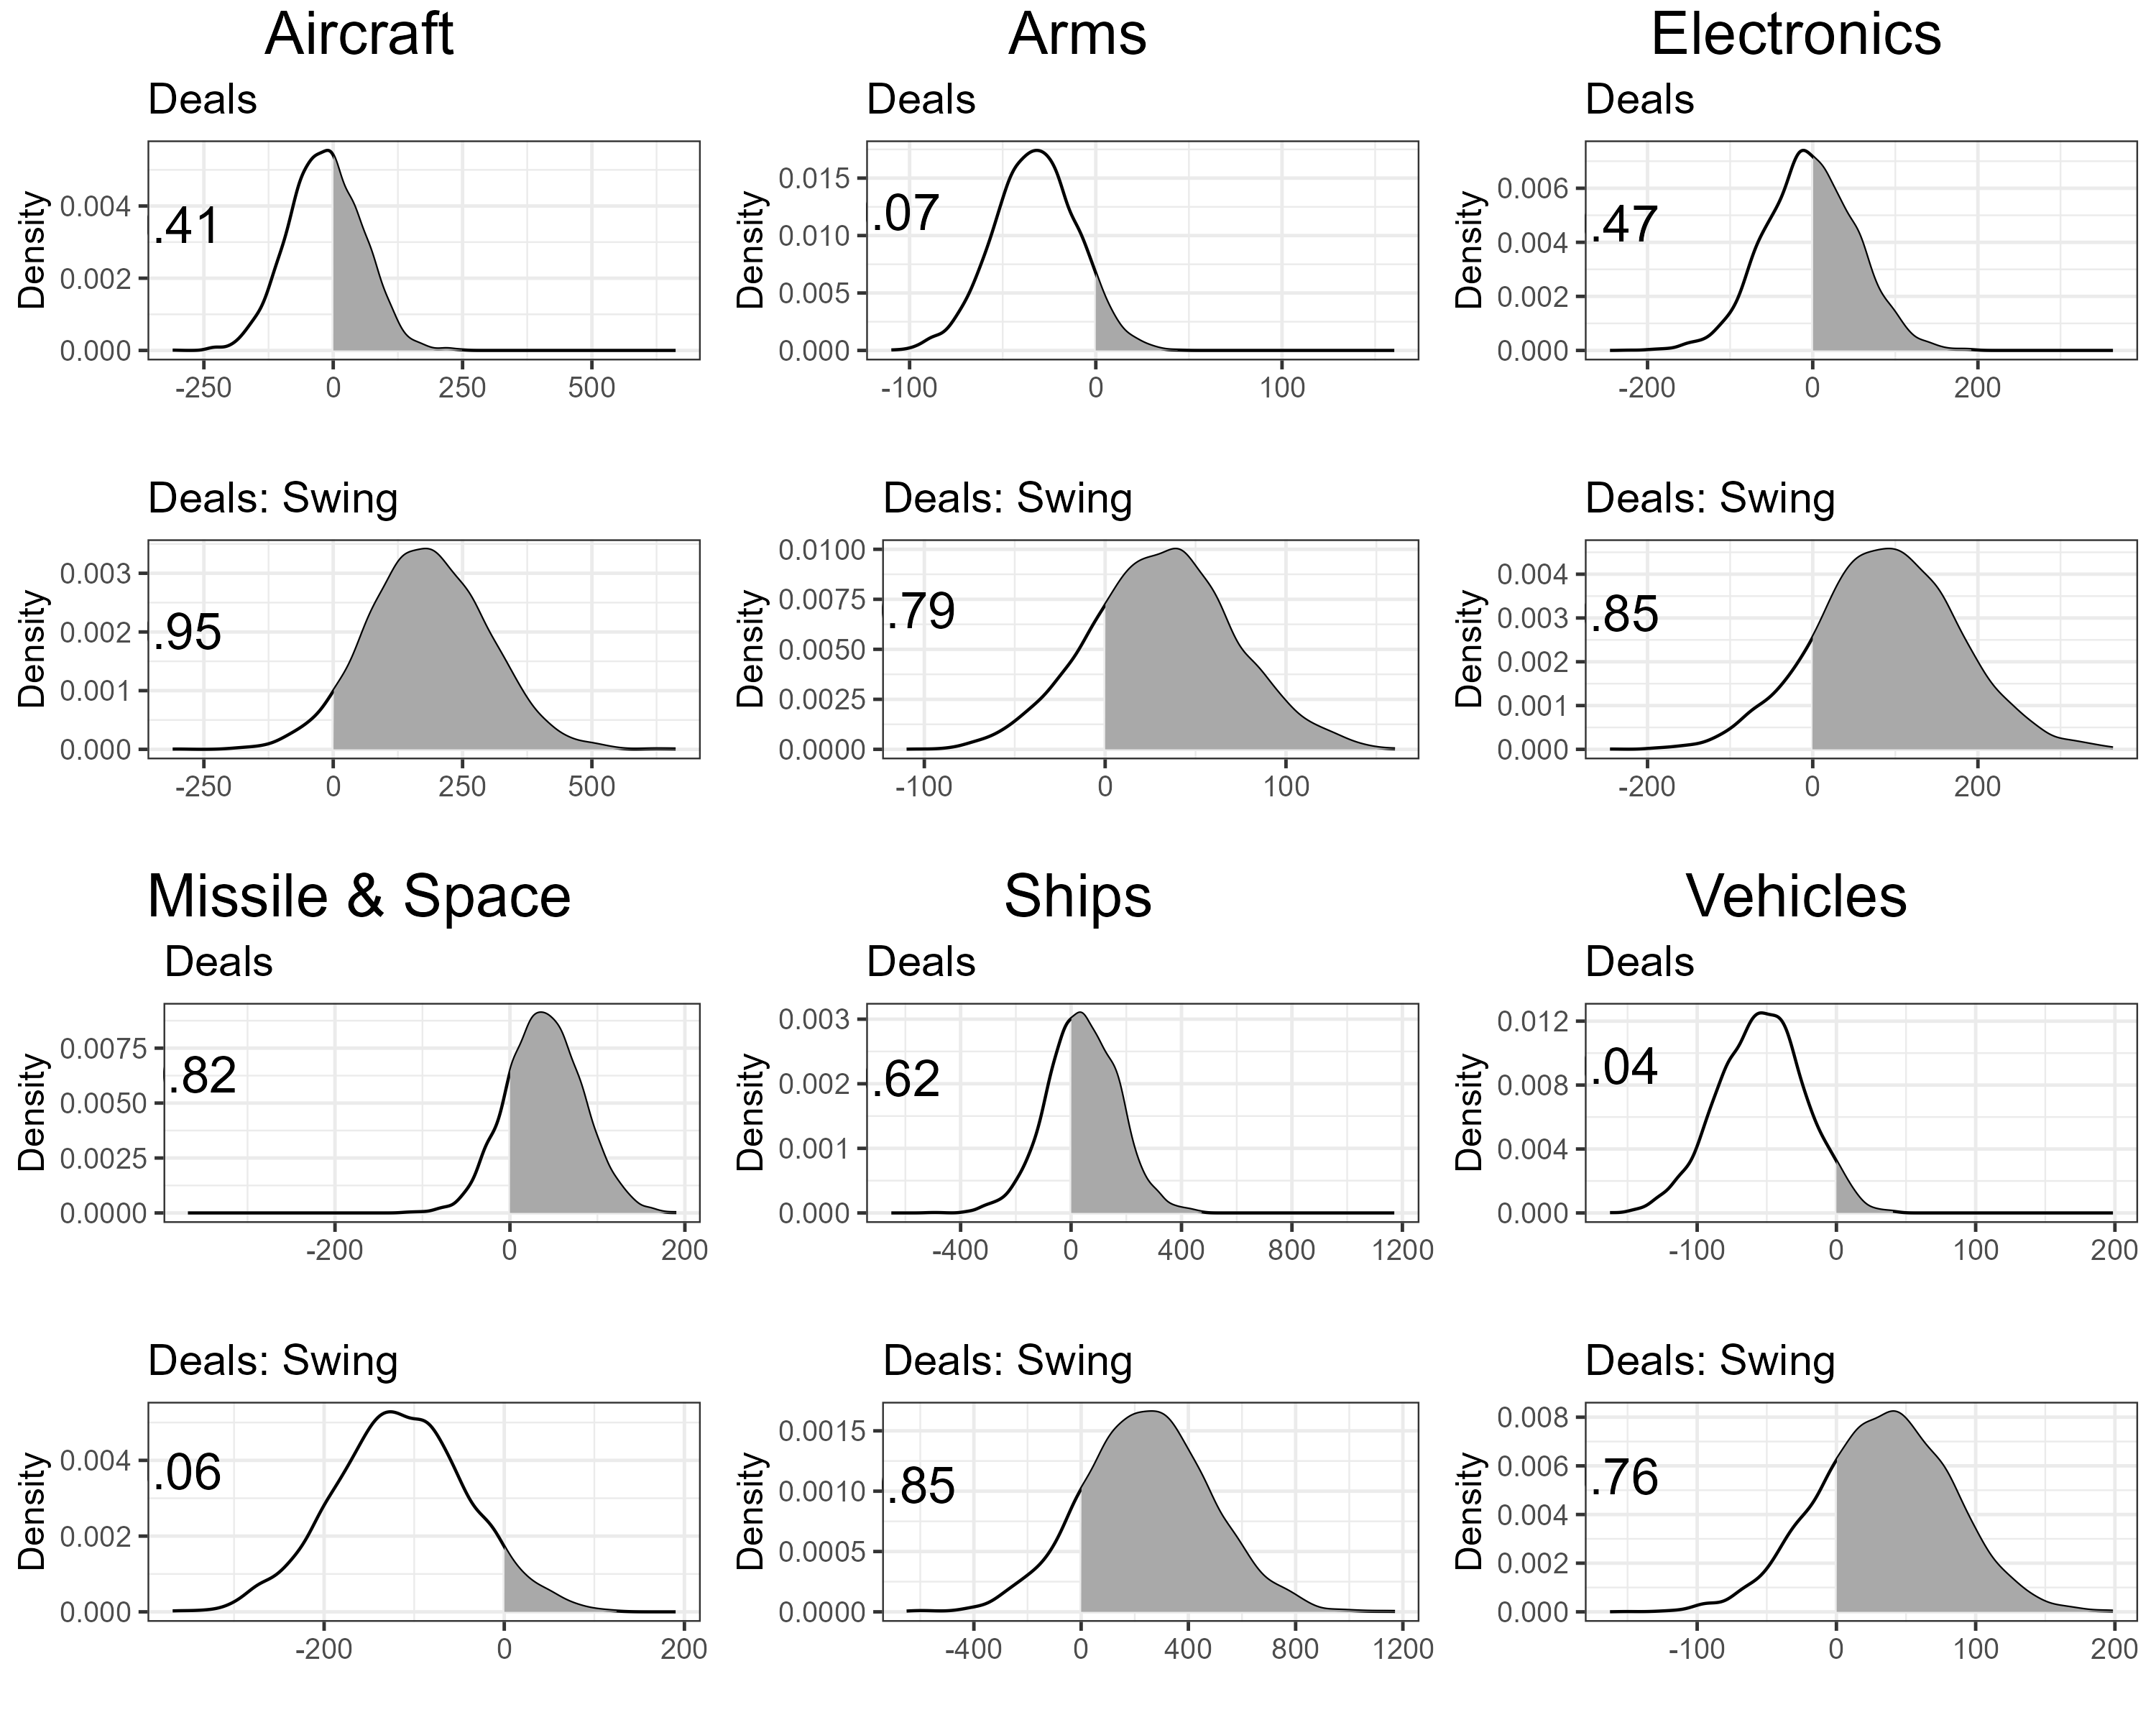
\includegraphics[width=0.95\textwidth]{../figures/me-deals-sector.png}
	\caption{Associations between different types of arms deals and defense contracts within defense industry sectors. Shaded area and text summarize the positive posterior mass. Estimates in millions of U.S. dollars.}
	\label{fig:me-deals-sector}
\end{figure}


While deals for most systems like arms, vehicles, and missile and space components have largely positive associations with related swing state contracts, aircraft deals have the greatest positive association. 
95\% of the posterior mass in the interaction of aircraft deals and swing state status is positive.
This probably reflects the diffuse aircraft supply chain, which incorporates engines, airframes, and other essential components. 


In addition to aircraft, ships and electronic deals are correlated with greater swing state contracts. 
Increases in ships deals are associated with \$300 million more contracts in a hypothetical swing state. 
Annual ships deals range from one to 11, so these deals are rare but lucrative. 
The impact also may not concentrate in shipyards, as most ships deals cover whole platforms, which require components from other regions. 

 
While electronics arms deals are less cyclical, most of the association between electronics deals and swing state contracts for military electronics is positive as well.
Electronics manufacturing does not come from electorally-driven arms deals, but electronics deals also feed swing state contracts. 
Similarly, much of the vehicles posterior mass is positive in swing states, though the direction of that association is less clear. 
Only missile and space production, which is geographically concentrated, has greater positive mass on the association between deals and contracts outside of swing states.


These results suggest that aircraft are the main component in arms deal cycles and aircraft deals often increase swing state contracts. 
Other deals in sectors like arms, electronics and ships may also increase swing state contracts, but these have less cyclical arms deals. 
Overall, this supports a connection between arms deals with autocratic allies and swing state contracts.  



\section{Discussion and Conclusion}


Arms deals with autocratic allies help U.S. leaders increase defense contracting awards in swing states. 
Arms deals with autocracies increase as presidential elections approach.
Deals then increase swing state contract awards. 
Much of this cooperation sends arms to autocratic U.S. allies like the Cold War era Brazilian junta and Saudi Arabia.


% alliance value and autoc alliance durability
This note helps explain why U.S. security cooperation with autocracies endures despite normative and practical criticisms. 
Arms deals increase autocratic allies' security and help U.S. leaders win elections.
While not a part of formal treaties, these informal linkages are essential to bargains between the United States and its security prot{\'e}g{\'e}s.
Electoral arms deals sustain regular cooperation across regimes.
%Allies need not undertake these cycles deliberately, but making arms deals is part of a cooperative bundle of ties.


In addition to helping explain U.S. security cooperation with autocracies, these findings add an international security component to the political budget cycle literature.
Alliance partnerships can help leaders manipulate economic conditions for electoral gain. 
By providing an outlet for defense contracting, allies help leaders award contracts with less attention to the budget process and force planning of the U.S. military.
The results also complement findings that states manipulate international economic ties to undermine adversarial leaders \citep{ChyzhUrbatsch2021, KimMargalit2021}, by showing how some partners aid cycles via security cooperation. 



Future research could proceed in several directions. 
Exploring the role of defense industry integration and intermediate goods in these arms cycles is potentially interesting.
Whether there are similar cycles outside the United States is also a worthy subject of future study. 
Other alliance patrons may take similar actions in different ways.


Electoral competition reshapes international security cooperation.
Efforts to use defense contracting to improve the economy in swing states encourage U.S. security cooperation with autocracies.
While these deals may empower states that misuse U.S. arms, electoral considerations take precedence. 


\newpage
\singlespace
 
\bibliography{../../MasterBibliography} 


\end{document}
